%%%%%%%%%%%%%%%%%%%%%%%%%%%%%%%%%%%%%%%%%%%%%%%%%%%%%%%%%%%%%%%%%%%%%%%%%%%%%%%%%%
\begin{frame}[fragile]\frametitle{}
\begin{center}
{\Large So, What (exactly) is AI?}
\end{center}
\end{frame}

%%%%%%%%%%%%%%%%%%%%%%%%%%%%%%%%%%%%%%%%%%%%%%%%%%%%%%%%%%%%%%%%%%%%%%%%%%%%%%%%%%
\begin{frame}[fragile]\frametitle{}
\begin{center}
(typical understanding)

{\Huge If Machines show intelligence, like Humans that's AI}
\end{center}
\end{frame}

%%%%%%%%%%%%%%%%%%%%%%%%%%%%%%%%%%%%%%%%%%%%%%%%%%%%%%%%%%
\begin{frame}[fragile]\frametitle{}
\begin{center}
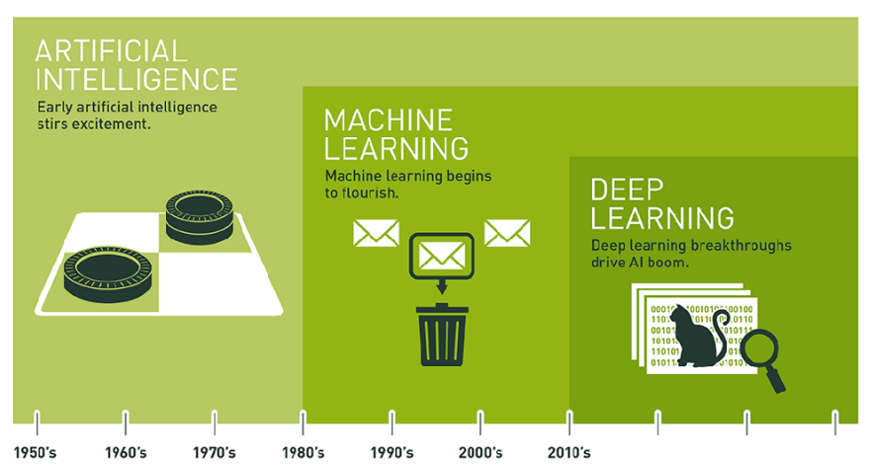
\includegraphics[width=\linewidth,keepaspectratio]{xai6}
\end{center}

\tiny{(Ref: Nvidia blog: Artificial Intelligence)}
\end{frame}

%%%%%%%%%%%%%%%%%%%%%%%%%%%%%%%%%%%%%%%%%%%%%%%%%%%%%%%%%%
\begin{frame}[fragile]\frametitle{Difference}
\begin{center}
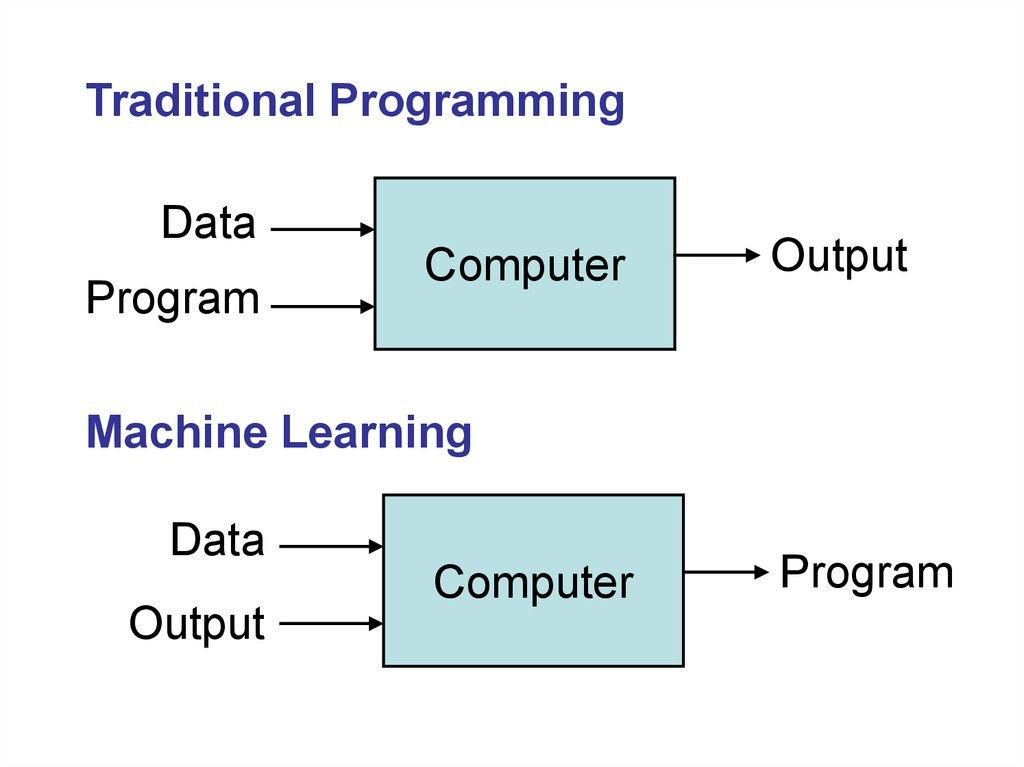
\includegraphics[width=0.8\linewidth,keepaspectratio]{xai7}
\end{center}

\tiny{(Ref: Machine Learning - Luis Serrano - Youtube)}
\end{frame}

%%%%%%%%%%%%%%%%%%%%%%%%%%%%%%%%%%%%%%%%%%%%%%%%%%%%%%%%%%
\begin{frame}[fragile]\frametitle{Supervised: Linear}
\begin{center}
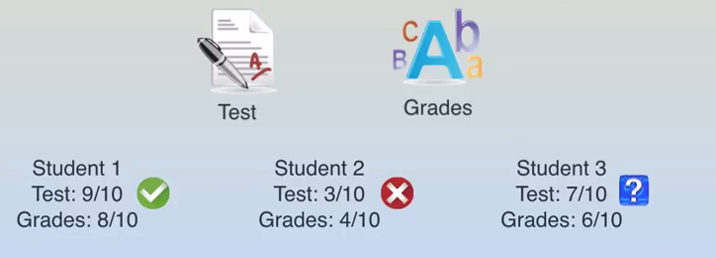
\includegraphics[width=\linewidth,keepaspectratio]{xai8}
\end{center}

\tiny{(Ref: Machine Learning - Luis Serrano - Youtube)}
\end{frame}

%%%%%%%%%%%%%%%%%%%%%%%%%%%%%%%%%%%%%%%%%%%%%%%%%%%%%%%%%%
\begin{frame}[fragile]\frametitle{Supervised: Linear}
\begin{center}
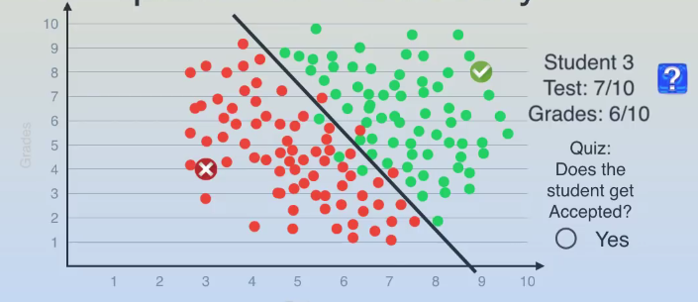
\includegraphics[width=\linewidth,keepaspectratio]{xai9}
\end{center}

\tiny{(Ref: Machine Learning - Luis Serrano - Youtube)}
\end{frame}

%%%%%%%%%%%%%%%%%%%%%%%%%%%%%%%%%%%%%%%%%%%%%%%%%%%%%%%%%%
\begin{frame}[fragile]\frametitle{Supervised: Non-Linear}
\begin{center}
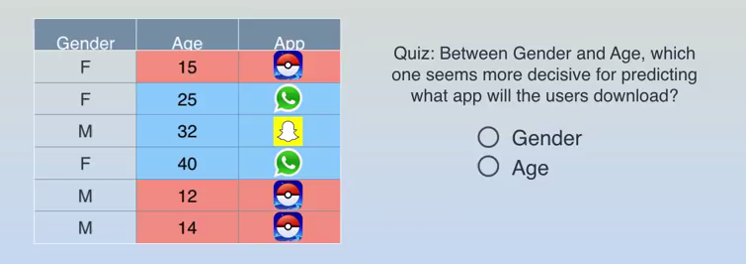
\includegraphics[width=\linewidth,keepaspectratio]{xai10}
\end{center}

\tiny{(Ref: Machine Learning - Luis Serrano - Youtube)}
\end{frame}

%%%%%%%%%%%%%%%%%%%%%%%%%%%%%%%%%%%%%%%%%%%%%%%%%%%%%%%%%%
\begin{frame}[fragile]\frametitle{Supervised: Non-Linear}
\begin{center}
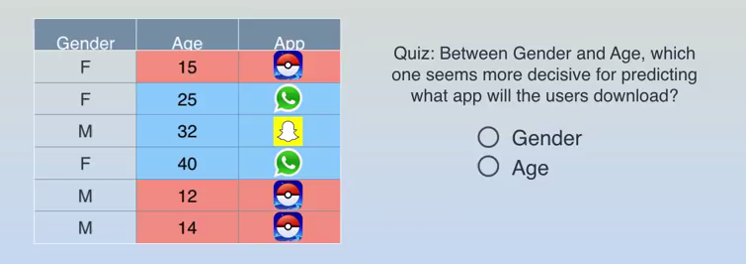
\includegraphics[width=\linewidth,keepaspectratio]{xai10}
\end{center}

\tiny{(Ref: Machine Learning - Luis Serrano - Youtube)}
\end{frame}

%%%%%%%%%%%%%%%%%%%%%%%%%%%%%%%%%%%%%%%%%%%%%%%%%%%%%%%%%%
\begin{frame}[fragile]\frametitle{Unsupervised}
\begin{center}
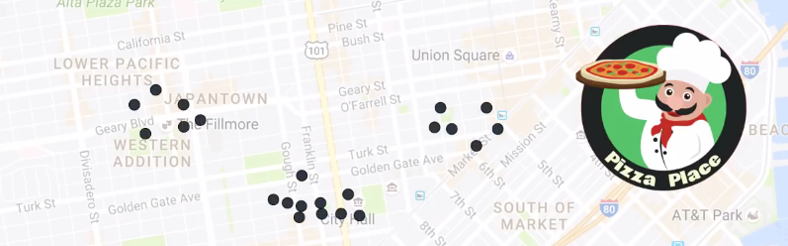
\includegraphics[width=\linewidth,keepaspectratio]{xai11}
\end{center}

\tiny{(Ref: Machine Learning - Luis Serrano - Youtube)}
\end{frame}

%%%%%%%%%%%%%%%%%%%%%%%%%%%%%%%%%%%%%%%%%%%%%%%%%%%%%%%%%%
\begin{frame}[fragile]\frametitle{Unsupervised}
\begin{center}
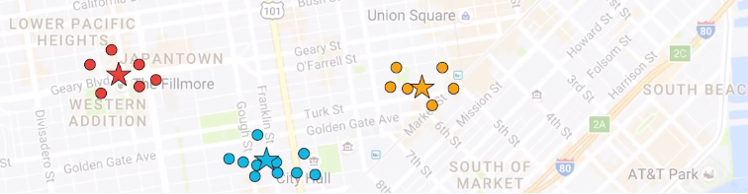
\includegraphics[width=\linewidth,keepaspectratio]{xai12}
\end{center}

\tiny{(Ref: Machine Learning - Luis Serrano - Youtube)}
\end{frame}

%%%%%%%%%%%%%%%%%%%%%%%%%%%%%%%%%%%%%%%%%%%%%%%%%%%%%%%%%%
\begin{frame}[fragile]\frametitle{How Neural Networks capture Non-Linearity?}
\begin{center}
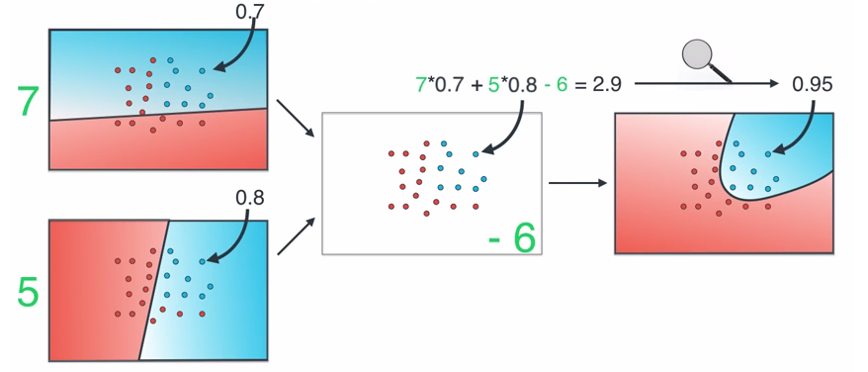
\includegraphics[width=\linewidth,keepaspectratio]{xai13}
\end{center}

\tiny{(Ref: Machine Learning - Luis Serrano - Youtube)}
\end{frame}

%%%%%%%%%%%%%%%%%%%%%%%%%%%%%%%%%%%%%%%%%%%%%%%%%%%%%%%%%%
\begin{frame}[fragile]\frametitle{How Neural Networks capture Non-Linearity?}
\begin{center}
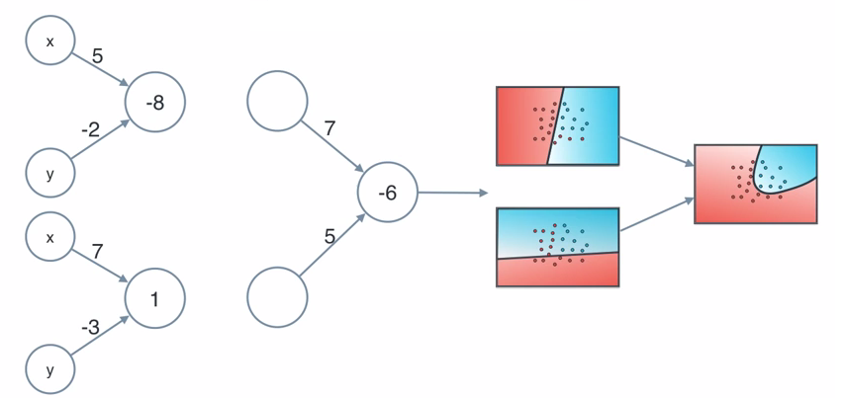
\includegraphics[width=\linewidth,keepaspectratio]{xai14}
\end{center}

\tiny{(Ref: Machine Learning - Luis Serrano - Youtube)}
\end{frame}

%%%%%%%%%%%%%%%%%%%%%%%%%%%%%%%%%%%%%%%%%%%%%%%%%%%%%%%%%%
\begin{frame}[fragile]\frametitle{How Neural Networks capture Non-Linearity?}
\begin{center}
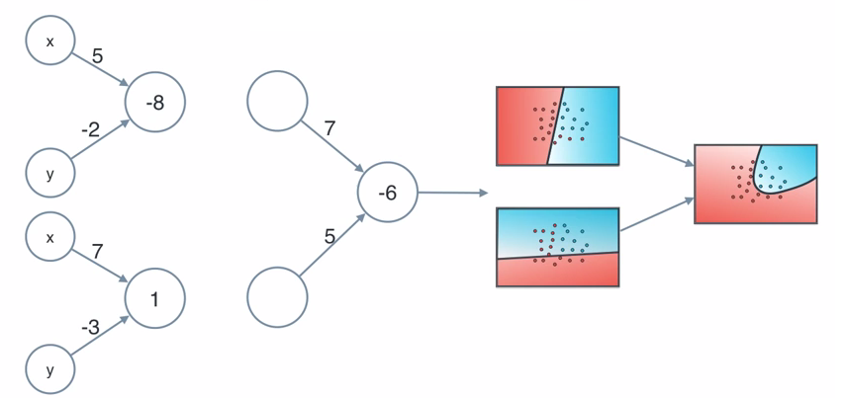
\includegraphics[width=\linewidth,keepaspectratio]{xai14}
\end{center}

\tiny{(Ref: Machine Learning - Luis Serrano - Youtube)}
\end{frame}

%%%%%%%%%%%%%%%%%%%%%%%%%%%%%%%%%%%%%%%%%%%%%%%%%%%%%%%%%%
\begin{frame}[fragile]\frametitle{How Neural Networks capture Non-Linearity?}
\begin{center}
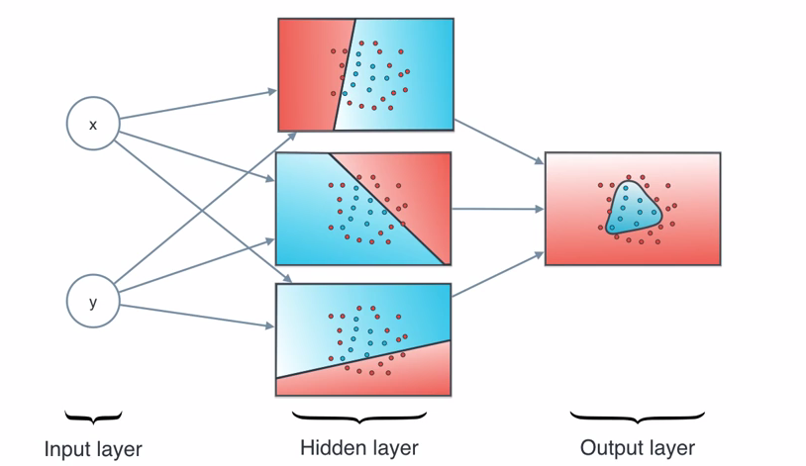
\includegraphics[width=\linewidth,keepaspectratio]{xai15}
\end{center}

\tiny{(Ref: Machine Learning - Luis Serrano - Youtube)}
\end{frame}

%%%%%%%%%%%%%%%%%%%%%%%%%%%%%%%%%%%%%%%%%%%%%%%%%%%%%%%%%%
\begin{frame}[fragile]\frametitle{The Whole Work-flow}
\begin{center}
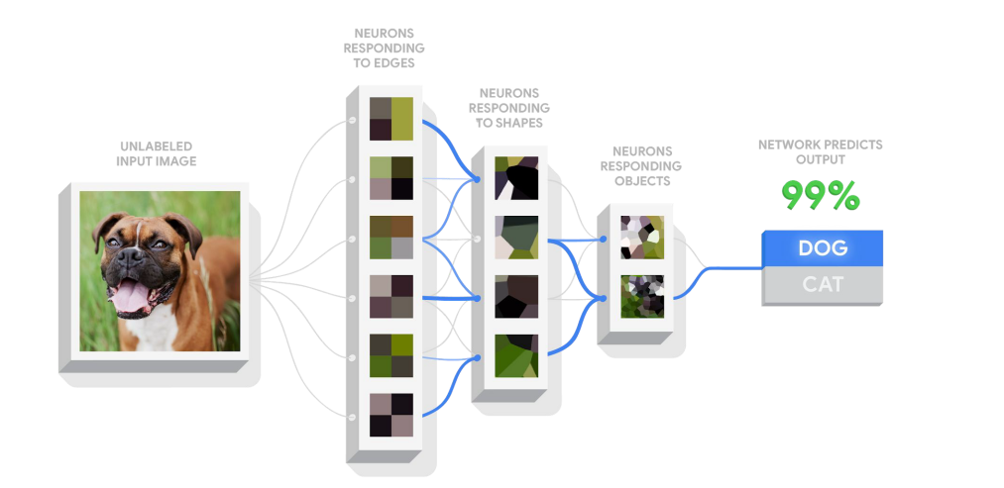
\includegraphics[width=\linewidth,keepaspectratio]{xai16}
\end{center}

\end{frame}

%%%%%%%%%%%%%%%%%%%%%%%%%%%%%%%%%%%%%%%%%%%%%%%%%%%%%%%%%%%
\begin{frame}[fragile]\frametitle{Explain-ability of AI Algorithms}
\begin{itemize}
\item {\bf Regression}: Multinomial Equation can be messy 
\item {\bf Random Forrest}: Multiple Tree and their Data Set and Voting 
\item {\bf SVM}: Kernel and Data Partition effect on Feature 
\item {\bf K Means}: Nature of Centroid don't describe cluster well. 
\item {\bf NN}: Hidden Nodes and their way of creating features 
\end{itemize}

\tiny{(Ref:Explainable AI (XAI) – A Perspective, Saurabh Kaushik  )}

\end{frame}

%%%%%%%%%%%%%%%%%%%%%%%%%%%%%%%%%%%%%%%%%%%%%%%%%%%%%%%%%%
\begin{frame}[fragile]\frametitle{But \ldots}
\begin{center}
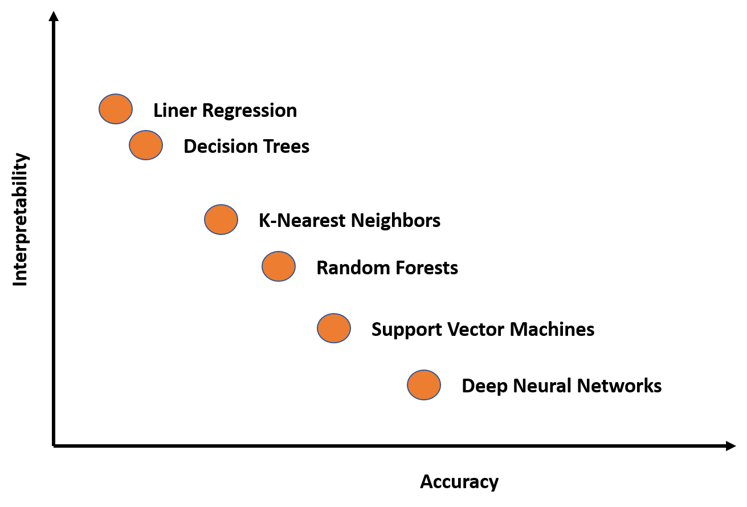
\includegraphics[width=0.8\linewidth,keepaspectratio]{xai17}
\end{center}

\tiny{(Ref: Application of artificial intelligence in gastroenterology, April 2019,World Journal of Gastroenterology 25(14):1666-1683)
}
\end{frame}

